\section{The DSLTrans Transformation Language}
\label{sec:dsltrans}

In this section we will introduce the DSLTrans transformation language and its
constructs from~\cite{DBLP:conf/sle/BarrocaLAFS10}. A formal treatment of the syntax and semantics of DSLTrans is found in \cref{sec:DSLTrans_formal_appendix}.

\reviewer{Please explain, earlier on, the meaning of indirect edges.}


\begin{figure*}[t]
        \centering
        \begin{subfigure}[b]{0.40\textwidth}
                \centering
                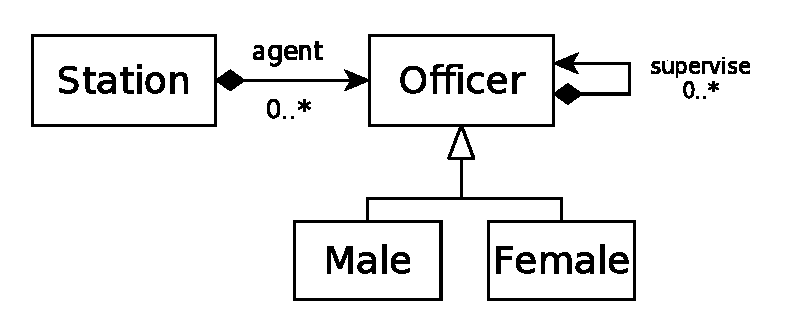
\includegraphics[width=1\textwidth]{./figures/policestation_dsltrans/organization.pdf}
                \caption{Organization language}
                \label{fig:OrganizationLanguage}
        \end{subfigure}%
        ~~
        \begin{subfigure}[b]{0.40\textwidth}
                \centering
                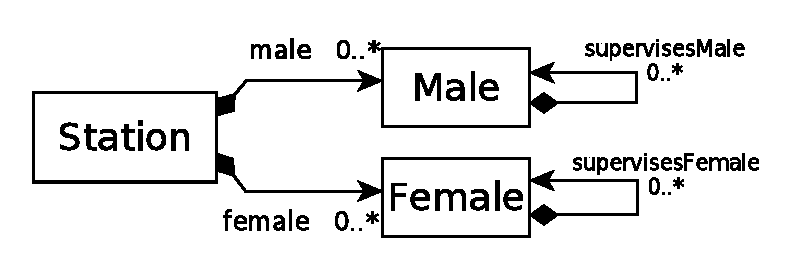
\includegraphics[width=1\textwidth]{./figures/policestation_dsltrans/gender.pdf}
                \caption{Gender language}
                \label{fig:GenderLanguage}
        \end{subfigure}%
        \caption{Metamodels for the Police Station transformation}
        \label{fig:squadmetamodel}
\end{figure*}

A DSLTrans transformation has a source and a target metamodel, which are seen
in \cref{fig:squadmetamodel}. This \emph{Police Station}
transformation will be presented throughout
the rest of this paper as an example transformation. The metamodel
in \cref{fig:OrganizationLanguage} represents a language for describing
the chain of command in a police station, which includes the male (\emph{Male}
class) and female officers (\emph{Female} class). The metamodel in
\cref{fig:GenderLanguage} represents a language for describing a different
view over the chain of command, where the officers working at the police station
are classified by gender.

\begin{figure*}[bht]
	\centering
		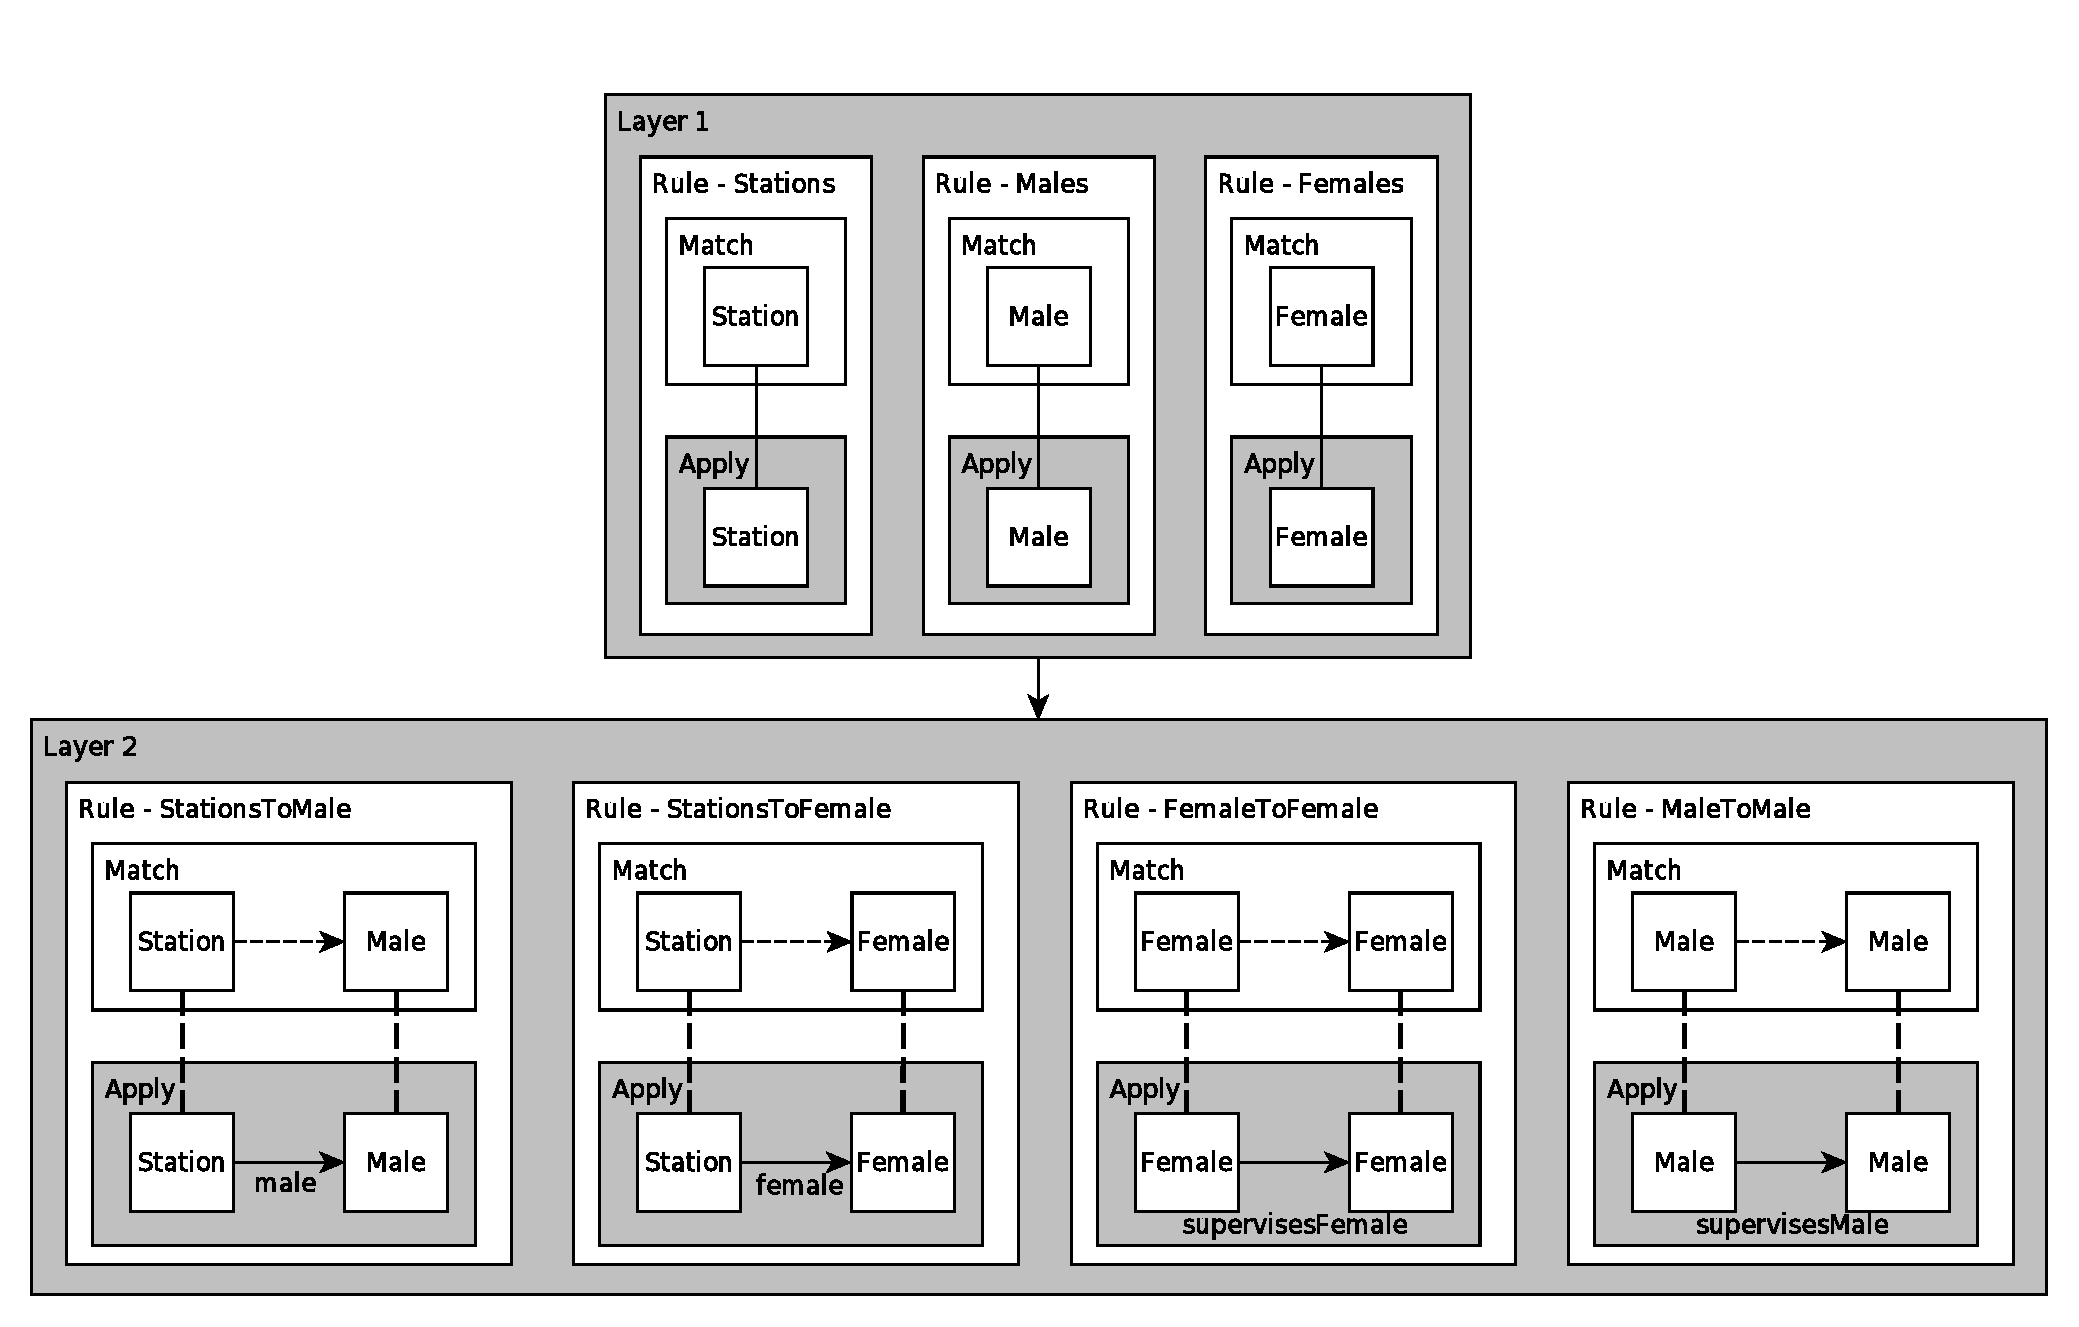
\includegraphics[width=0.9\textwidth]{./figures/policestation_dsltrans/transformation.pdf}
	\caption{The \emph{Police Station} model transformation expressed in DSLTrans}
	\label{fig:dsltransformation}
\end{figure*}

In \cref{fig:dsltransformation} we present a DSLTrans transformation that involves both metamodels.  A description of relevant constructs as well as visual notation remarks are found in \cref{subsec:DSLTrans_constructs}. Note
that the transformation is formed
from layers where each layer is a set of transformation rules. The
transformation will execute layer-by-layer, where transformation rules in a layer will execute in a
non-deterministic order but will always produce a deterministic result, due to the fact that DSLTrans is confluent by construction~\cite{DBLP:conf/sle/BarrocaLAFS10}.

Another important characteristic of DSLTrans transformations is that they are not Turing-complete. As discussed in~\cite{DBLP:conf/sle/BarrocaLAFS10}, non-completeness is required to make a transformation execution always terminate, but yet still allows for appropriate expressiveness.

Besides the fact that DSLTrans' transformations are free of constructs that
imply unbounded recursion or \\non-determinism, DSLTrans' transformations are strictly outplace, meaning no changes are allowed to the input model. However, the output metamodel for a DSLTrans transformation can
be the same as the input metamodel. Also, elements cannot be removed
from the output metamodel as the result of applying a DSLTrans rule.
This restriction is consistent with the usage of model transformations as
translations~\cite{AMT2012}, as no deletion of output elements is strictly required.

The purpose of this \emph{Police Station} transformation is to flatten a chain of command given
in the \emph{Organization language} into two independent sets of male
and female officers represented in the \emph{Gender language}. The command
relations will be kept during this transformation, i.e. a female officer will
have a direct association to all her female subordinates and likewise for male
officers. Note that differences in the gender classification metamodel mean
some relations present in the input model will not be retained in the output
model.

\begin{figure*}[htb]
        \centering
        \begin{subfigure}[b]{0.30\textwidth}
                \centering
                \includegraphics[width=1\textwidth]{./figures/policestation_dsltrans/model_police_hierarchy.pdf}
                \caption{Original model}
                \label{fig:police_hierarchy}
        \end{subfigure}%
        ~~
        \begin{subfigure}[b]{0.40\textwidth}
                \centering
                \includegraphics[width=1\textwidth]{./figures/policestation_dsltrans/model_police_gender.pdf}
                \caption{Transformed model}
                \label{fig:police_gender}
        \end{subfigure}%
        \caption{Model before and after transformation}
        \label{fig:transformationexample}
\end{figure*}
\reviewer{Figure 3: I would suggest adding another node f5 superviesd by f4, to illustrate the
notion of transitive closure. Another remark: I think the black containment dia-
monds do not belong in an instance model, as they are a metamodel notion.}

An example of this transformation's execution can be observed in \cref{fig:transformationexample}, where the input model is on the left and the output model is on the right. Notice that the elements $s$, $m_k$  and $f_k$ in \cref{fig:OrganizationLanguage} are instances of the source \emph{Organization} metamodel elements $Station$, $Male$ and $Female$ respectively. The primed elements in \cref{fig:police_gender} are their counterpart instances in the target \emph{Gender} metamodel.

Each individual transformation rule in the transformation is composed of two graphs. The first graph
is denoted as the \emph{match graph}, and is a pattern holding elements from the
source metamodel. Likewise, the \emph{apply graph} is a pattern containing
elements from the target metamodel. A formal definition of a transformation rule is found in~\cref{def:transformation_rule} in \cref{sec:formal_background}.

As an example, consider the transformation rule marked \emph{Stations} in the
first rule layer in \cref{fig:dsltransformation}. The match graph holds
one \emph{Station} element from the source metamodel, while the apply graph
holds one \emph{Station} element from the target metamodel. This means that for all
elements in the input model which are of type \emph{Station} in the
\emph{Organization Language}, an element of type
\emph{Station} in the \emph{Gender Language} will be created in the output model.

Note that in our approach, we require that the match graph of a rule is not a subgraph of the match graph of any other rule (as formally stated in \cref{def:layer_transformation} of model transformation, in \cref{sec:formal_background} of this paper). This requirement is to prevent the case where a rule could not execute independently of another rule, except for the cases when such dependency is explicitly defined by backward links. This is undesirable for the algorithm as presented here as we will explain later. However, as seen in~\cite{conf/gg/SelimLCDO14}, the expressiveness of the transformations our algorithm can examine \reviewer{Perhaps 'the expressiveness of the rule language'?}  is not restricted. In that work, we detail an operational rule processing step to handle overlapping rules.

\reviewer{In page 10 (answer to the reviewers) you say that rules for a 
  layer must be parallel independent. Is this written anywhere in the
  main part of the paper? }

\subsection{Properties to Prove}

The properties we aim to prove on the Police Station transformation are structural properties. These properties are composed of a pre-condition and a post-condition component, as seen in \cref{fig:properties}. 

Informally, a property can be read as `if the pre-condition graph matches on the input model to the transformation, then the post-condition graph will match any output model produced'. Further details as well as formal validity and completeness of the property proving process are discussed in \cref{sec:verif_dsltrans_props}.

As a brief example of property syntax and semantics, consider the property in \cref{fig:dsltrans_prop1}. The pre-condition graph is composed of a Station element connected to a Female element and a Male element, where all elements are from the \emph{Organization language} metamodel. This structure is repeated in the post-condition graph, with the difference that the metamodel for these elements is the \emph{Gender language}. Thus, this property represents the statement ``\emph{a model which includes a
police station that has both male and female officers will be
transformed into a model where the male officer will exist in the male set
and the female officer will exist in the female set}''. We expect this property to always hold in our transformation.

\begin{figure*}[thb]
        \centering
        \begin{subfigure}[b]{0.45\textwidth}
                \centering
                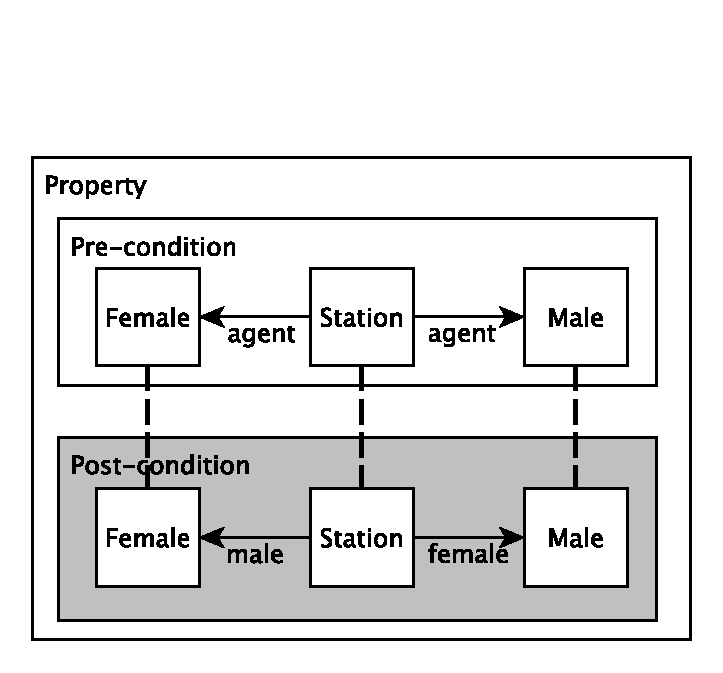
\includegraphics[height=5.5cm]{./figures/policestation_dsltrans/property1.pdf}
                \caption{Property 1 -- Expected to hold}
                \label{fig:dsltrans_prop1}
        \end{subfigure}%
        ~~
        \begin{subfigure}[b]{0.45\textwidth}
                \centering
                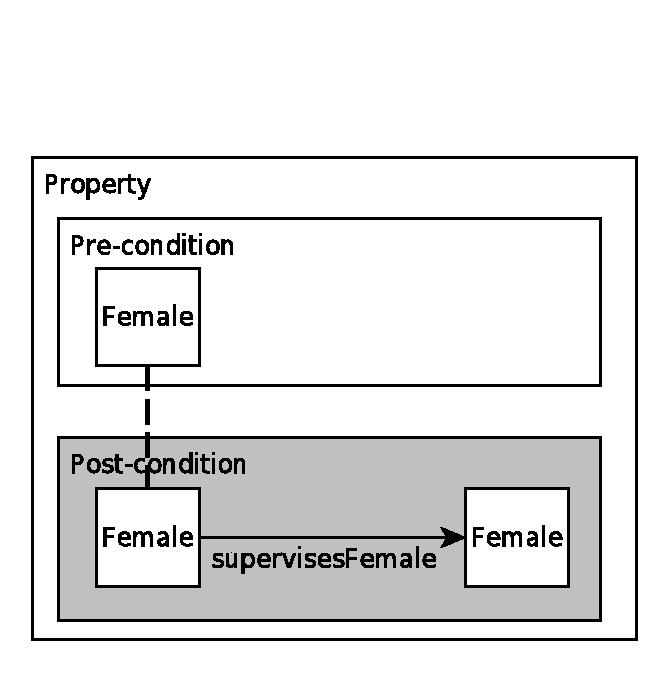
\includegraphics[height=5.5cm]{./figures/policestation_dsltrans/property2.pdf}
                \caption{Property 2 -- Not expected to hold}
                \label{fig:dsltrans_prop2}
        \end{subfigure}%
        \caption{ Properties to be proved on the Police Station transformation}
        \label{fig:properties}
\end{figure*}

\reviewer{Figure 4: The two “agent” edges in the postcondition should be marked “female”
resp. “male”} 
In contrast, we do not expect the property in \cref{fig:dsltrans_prop2} to always hold. This property represents the statement ``\emph{any model which includes a
female officer will be transformed into a model where that female officer will
always supervise another female officer}''. It is not difficult to construct an input model where the pre-condition holds, but the post-condition does not. For example, take an input model that contains only one female officer, as there will only be one female officer in the output model.

We shall discuss our property proving technique in \cref{sec:verif_dsltrans_props}. Following this, experiments in \cref{sec:experiments} will present experimental results from proving these two properties on the Police Station transformation.





\subsection{DSLTrans Constructs}
\label{subsec:DSLTrans_constructs}
This section will describe all of the DSLTrans constructs involved in our
property-proving algorithm. These constructs are found in the transformation presented in \cref{fig:dsltransformation}. Formal details for the handled constructs are found in \cref{sec:DSLTrans_formal} and \cref{sec:DSLTrans_syntax}, while \cref{sec:DSLTrans_semantics} briefly introduces the formal semantics of this subset of DSLTrans. The visual syntax presented here is based on the DSLTrans Eclipse plug-in syntax~\cite{dsltrans_manual}.

\begin{itemize}
\item \textbf{Match Elements}: Match elements are variables typed by elements of the source
metamodel which will match over elements of that type (or subtype) in the
input model when the transformation is executed. Note that match
elements in a rule are searched for injectively in a model. This means that, for
example, if a match graph includes two elements of type \emph{Station}, then the rule will only match over models that include at least two instances of type \emph{Station}.

In the DSLTrans notation as seen throughout this paper, the match elements will be in a white box in the top half of a rule.\\

\item \textbf{Direct Match Links}: Direct match links are variables typed by labelled associations of the source metamodel, which will match over associations of the same type in the input model. A direct match link is always expressed between two match elements.\\

\item \textbf{Indirect Match Links}: Indirect match links are similar to direct
match links, but there may exist a path of containment associations between the
matched instances. Our notion of indirect links captures only
acyclic EMF containment associations. \reviewer{“a nonempty path” (I think). The label of the
containment associations does not matter?}

% As such, it avoids cycles and infinite
% amounts of matches over the transitive closure of associations in the input
% models.

In \cref{fig:dsltransformation}, indirect match links are represented in all the
transformation rules in the last layer as dashed arrows between elements in the match graph.\\

\item \textbf{Backward Links}: Backward links connect elements of the match and
the apply patterns of a DSLTrans rule in order to represent dependencies on
element creation by previous layers of the transformation. When used in a rule,
backward links match over traceability links between elements of the
transformation's input and output models.
These traceability links are implicitly created when any rule is executed during the transformation. Backward
links thus make it possible to refer in a rule to output elements created by a
previous layer.

Backward links are found in \cref{fig:dsltransformation} in all transformation rules on the last layer and are depicted as dashed lines.\\

%\item \emph{Negative Conditions}: it is possible to express negative conditions over
%match elements, backward, direct and indirect match links. 

\item \textbf{Apply Elements and Apply Links}: Apply elements and apply links are similar to match elements and
match links, but are instead typed by elements of the target metamodel. Apply elements in a given transformation rule that are not connected to backward links will create elements of the same type in the transformation's output. Apply links will always be created in the transformation's output. These output elements and links will be created as many times as the match graph of the rule is isomorphically found in the input model.\\

Consider the transformation rule denoted \emph{Station2Male} in the last rule
layer of \cref{fig:dsltransformation}. This rule takes \emph{Station} and
\emph{Male} elements of the \emph{Gender Language} metamodel, where these
elements were created in a previous layer from \emph{Station} and \emph{Male}
elements of the \emph{Organization Language} metamodel, and connects them using a
\emph{male} association.

%\item \emph{Apply Attributes}: DSLTrans includes a small language for
%building the values attributes of apply model elements from references to one or
%more match model element attributes.
\end{itemize}


